\chapter{Background} 
\label{ch:background}

In this chapter, we describe the background of our research, 
including the basic technology related to this work, the 
hardware and software tools that we used to implement and evaluate 
our proposed algorithms in this work.


\section{White Space Bands}

The white space band term is mentioned the frequencies channels 
previously used by analog TV broadcasts. In United States, full 
power analog television broadcasts, which operated between the 
54 MHz and 806 MHz television frequencies (Channels 2-69), ceased 
operating on June 12, 2009 per a United States digital switchover 
mandate. At that time, full power TV stations were required to 
switch to digital transmission and operate only between 54 MHz 
and 698 MHz.~\cite{fccwhitespace} 

Industry and academia have recognized the value of white space 
bands in wireless communication. Various proposals, including 
IEEE 802.11af, IEEE 802.22 and those from the White Spaces 
Coalition, have advocated using white spaces left by the termination 
of analog TV to provide wireless broadband Internet access. Some 
company from industry has designed device intended to use these 
new available channels as a "white-spaces device" (WSD), such as 
Ubiquiti SR serials products. These devices are designed to detect 
the presence of existing but unused areas of airwaves, such as 
those reserved for analog television, and utilize these unused 
airwaves to transmit signals for data traffic. Such technology 
is predicted to improve the availability of broadband Internet 
service, especially in rural areas.

White space bands and ISM WiFi bands have great variation of 
propagation characteristics. Wireless propagation refers to 
the signal loss characteristics when wireless signals are 
transmitted through the wireless medium. The strength of the 
received signal depends on both the line-of-sight path (or lack 
thereof) and multiple other paths that result from reflection, 
diffraction, and scattering from obstacles~\cite{andersen1995propagation}. 
The widely-used Friis equation characterizes the received signal 
power $P_r$ in terms of transmit power $P_t$, transmitter gain 
$G_t$, receiver gain $G_r$, wavelength $\lambda$ of the carrier 
frequency, distance $R$ from transmitter to receiver, and path 
loss exponent $n$ according to~\cite{friis}:

\begin{equation}
\label{eq:friis}
P_r=P_t+G_t+G_r+10n \log_{10}\left( \frac{\lambda}{4\pi R}\right)
\end{equation}
Here, $n$ varies according to the aforementioned environmental 
factors with a value ranging from two to five in typical outdoor 
settings~\cite{rappaport}.

According to Eq.~\ref{eq:friis} white space band not only provide more 
bandwidth for wireless communication, but also bring the diversity in 
transmission/interference range. Our algorithms and frameworks try to 
exploit white space bands advantages of link communication and network 
deployment through spectrum agility with WiFi bands.


\section{Spectrum Utilization}

When access a channel licensed by FCC, most of the time we could detect signals in the 
air from devices who share the channel. To represent the utilization level of a channel, 
we define \emph{activity level}, $A$, as the percentage of time when the channel is 
occupied by all competing sources $x_j (j = 1, 2, 3, ...)$ other than the intended 
transmitter $y$. For 802.11-based transmissions, the activity level on band $i$ is 
defined as:
\begin{equation}
\label{eqn:80211activity}
A^i = \frac{\sum_j{\sum_k{\frac{L_k^{x_j}}{R_k^{x_j}}}}}{\sum_k{\frac{L_k^y}{R_k^y}}+\sum_j{\sum_k{\frac{L_k^{x_j}}{R_k^{x_j}}}}+S\sigma}
\end{equation}
where $L_k^{x_j}$ and $R_k^{x_j}$ represent the packet length in bits and data
rate at which that packet is transmitted, for external sources $x_j$;
$S$ and $\sigma$ are the number of idle slots and slot duration, respectively. 
When considering the activity level of non-802.11 users 
({\it e.g.}, the bands currently licensed to TV),
we use the received signal level from non-802.11 interfering sources $P_N^i$ 
on band $i$ directly as an input to our algorithms. 


% Talk about the available channel
In practical, we get the activity level through in-field measurements.
The measurements process will be introduced in following chapters.
We define the percentage of sensing samples ($S_\theta$) above an 
interference threshold ($\theta$) over the total samples ($S$) in a time unit as the 
activity level ($A$) of inter-network interference:
\begin{equation}
\label{eq:actdef}
A=\frac{S_\theta}{S_a}
\end{equation}
The capacity of a clean channel is denoted by $C$. With the protocol model, the capacity 
of a channel with inter-network interference $C_r$ could be represented as 
the remaining free time of the channel capacity according to: 
\begin{equation}
\label{eq:intercap}
C_r=C*(1-\bar{A})
\end{equation}


\section{Gateworks Platform}

The off the shelf platform we use for our measurements is the GW2358. 
GW2358 is a member of the Gateworks Cambria Single Board Computer family. 
The GW2358 meets the requirements for enterprise and residential network 
applications. This single board computer consists of an Intel IXP435 XScale 
operating at 667MHz, 128Mbytes of DDRII-400 DRAM, and 32Mbytes of Flash. 
Peripherals include four Type III Mini-PCI sockets, two 10/100 Base-TX 
Ethernet ports with IEC-6100-4 ESD and EFT protection, two USB Host ports, 
and Compact Flash socket. Additional features include digital I/O, serial 
EEPROM, real time clock with battery backup, system monitor to track 
operating temperature and input voltage, RS232 serial port for management 
and debug, and watchdog timer. The GW2358 also supports GPS and RS485 
serial port as ordering options. Power is applied through a dedicated 
connector or through either Ethernet connector with the unused signal 
pairs in a passive power over Ethernet architecture. 
An open source software OpenWrt board support package is included 
for Linux operating systems.


\begin{figure} 
%\vspace{-0.1in}
\centering
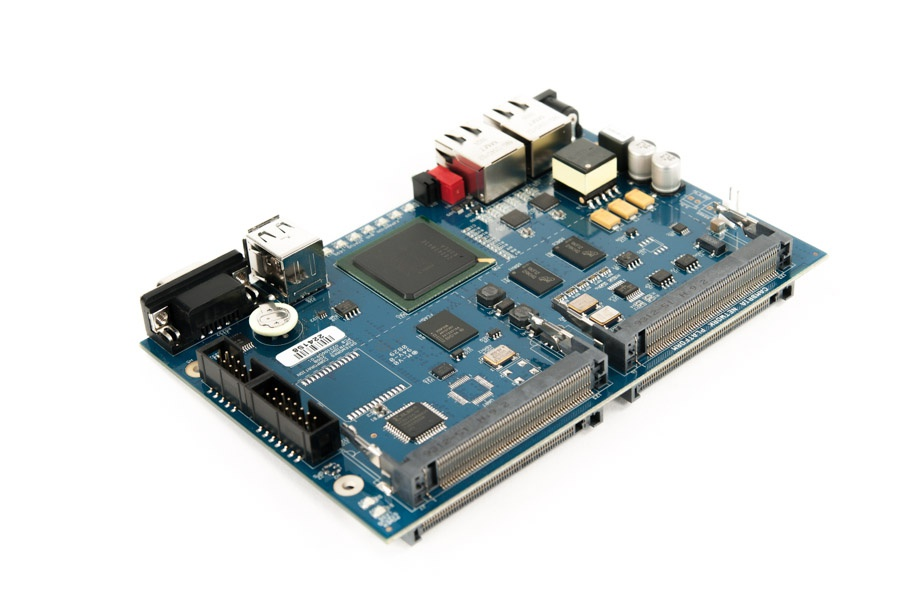
\includegraphics[width=75mm]{figures/gw2358}
\vspace{-0.1in}
\caption{The Gateworks GW2358 off-shelf Platform.}
\label{fig:gw2358}
\vspace{0.1in}
\end{figure}



The Gateworks platform works with Ubnt radios to perform 802.11 
multiband measurements for both indoor and in-field. It helps to 
collect the SNR, throughput and packet information for the post 
process. 

\section{Rohde \& Schwarz FSH8 Spectrum Analyzer}

The R\&S FSH 8 spectrum analyzer is designed portable for application 
in multiple environment, especially for in-field measurement. Its low 
weight, its simple, well-conceived operation concept and the large number 
of measurement functions make it an indispensable tool for anyone who 
needs an efficient measuring instrument for outdoor work. We employ 
FSH 8 in our indoor and outdoor measurements to collect data in multiple
bands.

\begin{figure} 
%\vspace{-0.1in}
\centering
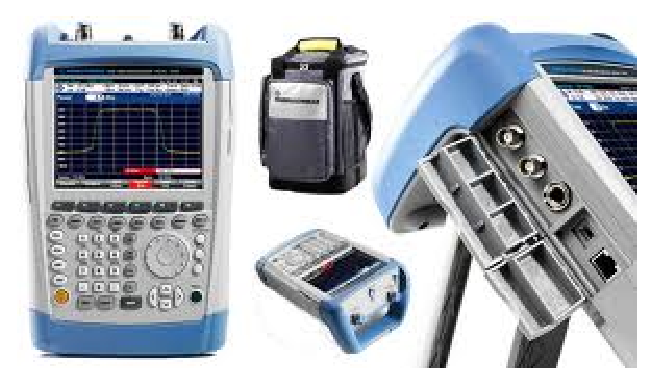
\includegraphics[width=75mm]{figures/fsh8}
\vspace{-0.1in}
\caption{Rohde \& Schwarz FSH 8 Spectrum Analyzer.}
\label{fig:fsh8}
\vspace{0.1in}
\end{figure}

FSH 8 is able to sense the signal in the air from 9 KHz to 
8 GHz. The spectrum analyzer could sense both 802.11 signals 
and non-802.11 signal in the air. Through the time stamp, 
we could merge data from Gateworks platform and FSH8 platform 
to perform our algorithms and frameworks.

\section{Mesh Network Deployment}

A wireless mesh network is a common infrastructure for providing 
wireless access for clients by the network carriers. Wireless 
mesh networks is made up of multiple radios which organize in a mesh 
topology. Each node forwards messages on behalf of the 
other nodes. The nodes connected to clients are referred to as the 
access tier. The nodes to relay data traffic to 
wired networks are referred to as the backhual tier. For the  access tier, the 
nodes need to cover the service area and provide sufficient 
capacity for the clients in target area. The backhual 
tier needs to have a highly-efficient path to the wired 
network which can potentially shorten multiple wireless hops. 
We analyze mesh network deployments in a scenario which includes multiple frequency bands, 
and propose our solutions for access and backhual 
network deployment.

